\documentclass{article}

\usepackage[inner=0.5cm,outer=0.5cm,top=1cm,bottom=0.5cm]{geometry}

\pagestyle{empty}
% This document contains the TikZ-header for all our LaTeX-computations.
% It especially contains all global graphic parameters.

\usepackage{amsmath, amssymb, amsfonts} % Standard Math-stuff

\usepackage{ifthen}

\usepackage{tikz}
\usetikzlibrary{calc}
\usetikzlibrary{positioning}
\usetikzlibrary{shapes}
\usetikzlibrary{patterns}


% Sometimes we want to implement different behaviour for the generated 
% HTML-pictures (for example, shading is not supported in HTML).
% For that we define a macro to check whether we run the code with
% htlatex. The code comes from 
% https://tex.stackexchange.com/questions/93852/what-is-the-correct-way-to-check-for-latex-pdflatex-and-html-in-the-same-latex
\makeatletter
\edef\texforht{TT\noexpand\fi
  \@ifpackageloaded{tex4ht}
    {\noexpand\iftrue}
    {\noexpand\iffalse}}
\makeatother


% Define a text=none option for nodes that ignores the given text, from
% https://tex.stackexchange.com/questions/59354/no-text-none-in-tikz
\makeatletter
\newif\iftikz@node@phantom
\tikzset{
  phantom/.is if=tikz@node@phantom,
  text/.code=%
    \edef\tikz@temp{#1}%
    \ifx\tikz@temp\tikz@nonetext
      \tikz@node@phantomtrue
    \else
      \tikz@node@phantomfalse
      \let\tikz@textcolor\tikz@temp
    \fi
}
\usepackage{etoolbox}
\patchcmd\tikz@fig@continue{\tikz@node@transformations}{%
  \iftikz@node@phantom
    \setbox\pgfnodeparttextbox\hbox{}
  \fi\tikz@node@transformations}{}{}
\makeatother

% Find the angle of a given line (within TikZ)
\newcommand{\tikzAngleOfLine}{\tikz@AngleOfLine}
\def\tikz@AngleOfLine(#1)(#2)#3{%
  \pgfmathanglebetweenpoints{%
    \pgfpointanchor{#1}{center}}{%
    \pgfpointanchor{#2}{center}}
  \pgfmathsetmacro{#3}{\pgfmathresult}%
}

% Now we define the global styles
% The global styles are defined nestedly. You have to give your tikzpicture
% the global options [vertexStyle, edgeStyle, faceStyle] to activate them.
% 
% You can disable labels by using the option nolabels, i.e. 
% vertexStyle=nolabels to deactivate vertex labels.
%
% If you want to have a specific style for your picture, you can also use
% this specific meta-style instead of the general style. For example if you
% want to use double edges in one single picture - no matter the style of
% the rest of the document - you can use edgeDouble instead of edgeStyle.
%
% To set the default style, modify the vertexStyle/.default entry.

% Vertex styles
\tikzset{ 
    vertexNodePlain/.style = {fill=#1, shape=circle, inner sep=0pt, minimum size=2pt, text=none},
    vertexNodePlain/.default=gray,
    vertexPlain/labels/.style = {
        vertexNode/.style={vertexNodePlain=##1},
        vertexLabel/.style={gray}
    },
    vertexPlain/nolabels/.style = {
        vertexNode/.style={vertexNodePlain=##1},
        vertexLabel/.style={text=none}
    },
    vertexPlain/.style = vertexPlain/#1,
    vertexPlain/.default=labels
}
\tikzset{
    vertexNodeNormal/.style = {fill=#1, shape=circle, inner sep=0pt, minimum size=4pt, text=none},
    vertexNodeNormal/.default = blue,
    vertexNormal/labels/.style = {
        vertexNode/.style={vertexNodeNormal=##1},
        vertexLabel/.style={blue}
    },
    vertexNormal/nolabels/.style = {
        vertexNode/.style={vertexNodeNormal=##1},
        vertexLabel/.style={text=none}
    },
    vertexNormal/.style = vertexNormal/#1,
    vertexNormal/.default=labels
}
\tikzset{
    vertexNodeBallShading/pdf/.style = {ball color=#1},
    vertexNodeBallShading/svg/.style = {fill=#1},
    vertexNodeBallShading/.code = {% Conditional shading depending whether we want pdf or svg output
        \if\texforht
            \tikzset{vertexNodeBallShading/svg=#1!90!black}
        \else
            \tikzset{vertexNodeBallShading/pdf=#1}
        \fi
    },
    vertexNodeBall/.style = {shape=circle, vertexNodeBallShading=#1, inner sep=2pt, outer sep=0pt, minimum size=3pt, font=\tiny},
    vertexNodeBall/.default = white,
    vertexBall/labels/.style = {
        vertexNode/.style={vertexNodeBall=##1, text=black},
        vertexLabel/.style={text=none}
    },
    vertexBall/nolabels/.style = {
        vertexNode/.style={vertexNodeBall=##1, text=none},
        vertexLabel/.style={text=none}
    },
    vertexBall/.style = vertexBall/#1,
    vertexBall/.default=labels
}
\tikzset{ 
    vertexStyle/.style={vertexNormal=#1},
    vertexStyle/.default = labels
}


% 1) optional: colour of vertex
% 2) position of the vertex
% 3) relative position of the node
% 4) name of the vertex
\newcommand{\vertexLabelR}[4][]{
    \ifthenelse{ \equal{#1}{} }
        { \node[vertexNode] at (#2) {#4}; }
        { \node[vertexNode=#1] at (#2) {#4}; }
    \node[vertexLabel, #3] at (#2) {#4};
}
% 1) optional: colour of vertex
% 2) position of the vertex
% 3) absolute position of the node
% 4) name of the vertex
\newcommand{\vertexLabelA}[4][]{
    \ifthenelse{ \equal{#1}{} }
        { \node[vertexNode] at (#2) {#4}; }
        { \node[vertexNode=#1] at (#2) {#4}; }
    \node[vertexLabel] at (#3) {#4};
}


% Edge styles
% If you have trouble with the double-lines overlapping, this might (?) help:
% https://tex.stackexchange.com/questions/288159/closing-the-ends-of-double-line-in-tikz
\newcommand{\edgeLabelColor}{blue!20!white}
\tikzset{
    edgeLineNone/.style = {draw=none},
    edgeLineNone/.default=black,
    edgeNone/labels/.style = {
        edge/.style = {edgeLineNone=##1},
        edgeLabel/.style = {fill=\edgeLabelColor,font=\small}
    },
    edgeNone/nolabels/.style = {
        edge/.style = {edgeLineNone=##1},
        edgeLabel/.style = {text=none}
    },
    edgeNone/.style = edgeNone/#1,
    edgeNone/.default = labels
}
\tikzset{
    edgeLinePlain/.style={line join=round, draw=#1},
    edgeLinePlain/.default=black,
    edgePlain/labels/.style = {
        edge/.style={edgeLinePlain=##1},
        edgeLabel/.style={fill=\edgeLabelColor,font=\small}
    },
    edgePlain/nolabels/.style = {
        edge/.style={edgeLinePlain=##1},
        edgeLabel/.style={text=none}
    },
    edgePlain/.style = edgePlain/#1,
    edgePlain/.default = labels
}
\tikzset{
    edgeLineDouble/.style = {very thin, double=#1, double distance=.8pt, line join=round},
    edgeLineDouble/.default=gray!90!white,
    edgeDouble/labels/.style = {
        edge/.style = {edgeLineDouble=##1},
        edgeLabel/.style = {fill=\edgeLabelColor,font=\small}
    },
    edgeDouble/nolabels/.style = {
        edge/.style = {edgeLineDouble=##1},
        edgeLabel/.style = {text=none}
    },
    edgeDouble/.style = edgeDouble/#1,
    edgeDouble/.default = labels
}
\tikzset{
    edgeStyle/.style = {edgePlain=#1},
    edgeStyle/.default = labels
}

% Face styles
% Here we have an exception - the style face is always defined.
% 
\newcommand{\faceColorY}{yellow!60!white}   % yellow
\newcommand{\faceColorB}{blue!60!white}     % blue
\newcommand{\faceColorC}{cyan!60}           % cyan
\newcommand{\faceColorR}{red!60!white}      % red
\newcommand{\faceColorG}{green!60!white}    % green
\newcommand{\faceColorO}{orange!50!yellow!70!white} % orange

% define default face colour (and default swap colour)
\newcommand{\faceColor}{\faceColorY}
\newcommand{\faceColorSwap}{\faceColorC}

% define secondary default colours (to use in a single section)
\newcommand{\faceColorFirst}{green!40!white}
\newcommand{\faceColorSecond}{gray!15!white}
\newcommand{\faceColorThird}{red!17!white}
\newcommand{\faceColorFourth}{olive!20!white}

\tikzset{
    face/.style = {fill=#1},
    face/.default = \faceColor,
    faceY/.style = {face=\faceColorY},
    faceB/.style = {face=\faceColorB},
    faceC/.style = {face=\faceColorC},
    faceR/.style = {face=\faceColorR},
    faceG/.style = {face=\faceColorG},
    faceO/.style = {face=\faceColorO}
}
\tikzset{
    faceStyle/labels/.style = {
        faceLabel/.style = {}
    },
    faceStyle/nolabels/.style = {
        faceLabel/.style = {text=none}
    },
    faceStyle/.style = faceStyle/#1,
    faceStyle/.default = labels
}
\tikzset{ face/.style={fill=#1} }
\tikzset{ faceSwap/.code=
    \ifdefined\swapColors
        \tikzset{face=\faceColorSwap}
    \else
        \tikzset{face=\faceColor}
    \fi
}



\usepackage{hyperref}


\begin{document}



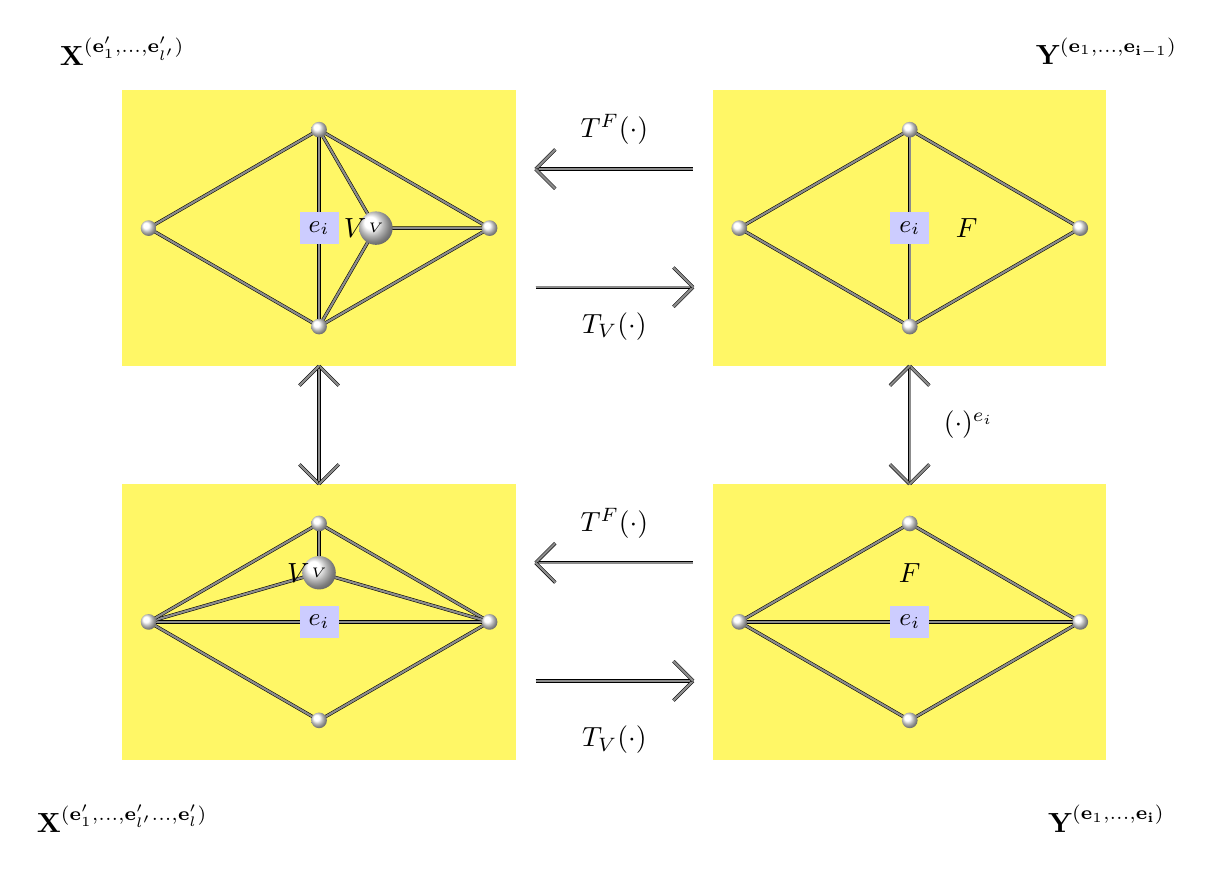
\begin{tikzpicture}[vertexBall, edgeDouble, faceStyle, scale=2.5]

% Define the coordinates of the vertices
\coordinate (V2_1) at (0, 0);
\coordinate (V3_1) at (0, 1);
\coordinate (V1_1) at (0.8660254037844386,0.4999999999999999);
\coordinate (V4_1) at (-0.8660254037844386,0.4999999999999999);
\coordinate (V1) at (barycentric cs:V2_1=1,V3_1=1,V1_1=1);
\coordinate (V2) at (-0.8660,0.5);


\coordinate (V2_2) at (3, 0);
\coordinate (V3_2) at (3, 1);
\coordinate (V1_2) at (3.8660254037844386,0.4999999999999999);
\coordinate (V4_2) at (-0.8660254037844386+3,0.4999999999999999);
\coordinate (V12) at (barycentric cs:V2_2=1,V3_2=1,V1_2=1);
\coordinate (V22) at (-0.8660+3,0.5);


\coordinate (V2_3) at (3, -2);
\coordinate (V3_3) at (3, -1);
\coordinate (V1_3) at (3.8660254037844386,0.4999999999999999-2);
\coordinate (V4_3) at (-0.8660254037844386+3,0.4999999999999999-2);
\coordinate (V13) at (barycentric cs:V2_3=1,V3_3=1,V1_3=1);
\coordinate (V23) at (-0.8660+3,0.5-2);

\coordinate (V2_4) at (0, -2);
\coordinate (V3_4) at (0, -1);
\coordinate (V1_4) at (0.8660254037844386,0.4999999999999999-2);
\coordinate (V4_4) at (-0.8660254037844386,0.4999999999999999-2);
\coordinate (V14) at (barycentric cs:V4_4=1,V3_4=2,V1_4=1);
\coordinate (V24) at (-0.8660,0.5-2);

% Fill in the faces
\fill[face]  (-1.,-0.2) -- (-1.,1.2) --(1,1.2) --(1,-0.2) -- cycle;
\fill[face]  (-1.,-0.2-2) -- (-1.,1.2-2) --(1,1.2-2) --(1,-0.2-2) -- cycle;
\fill[face]  (-1.+3,-0.2-2) -- (-1.+3,1.2-2) --(1+3,1.2-2) --(1+3,-0.2-2) -- cycle;
\fill[face]  (-1.+3,-0.2) -- (-1.+3,1.2) --(1+3,1.2) --(1+3,-0.2) -- cycle;
\fill[face]  (V2_1) -- (V3_1) -- (V1_1) -- cycle;
%\node[faceLabel] at (barycentric cs:V2_1=1,V3_1=1,V1_1=1) {$ $};
%\fill[face]  (V2_1) -- (V3_1) -- (V2) -- cycle;
\node[faceLabel] at (V12) {$ 
F$};
\node[faceLabel] at (barycentric cs:V23=1,V3_3=2,V1_3=1) {$ 
F$};
%\node[faceLabel] at (barycentric cs:V2_1=1,V3_1=1,V1=2) {$F_1 $};
%\node[faceLabel] at (barycentric cs:V2_1=1,V1_1=1,V1=2) {$F_3 $};
%\node[faceLabel] at (barycentric cs:V1_1=1,V3_1=1,V1=2) {$F_2 $};
%\node[faceLabel] at (barycentric cs:V2=2,V3_1=1,V4_1=1) {$f_3 $};
%\node[faceLabel] at (barycentric cs:V3_1=1,V2_1=1,V2=2) {$F'
%$};
\node[faceLabel] at (1.5,1.) {$T^F(\cdot) $};
\node[faceLabel] at (1.5,-2.1) {$T_V(\cdot) $};
\node[faceLabel] at (1.5,-0.) {$T_V(\cdot) $};
\node[faceLabel] at (1.5,-1.) {$T^F(\cdot) $};
\node[faceLabel] at (0.3+3,-0.5) {$(\cdot)^{e_i} $};
%\node[faceLabel] at (-.4,-0.5) {$(\cdot)^{\overline{E}} $};
\node[faceLabel] at (4,-2.5) {$\textbf{Y}^{(\textbf{e}_1,\ldots,\textbf{e}_\textbf{i})}$};

\node[faceLabel] at (4,1.4) {$\textbf{Y}^{(\textbf{e}_1,\ldots,\textbf{e}_{\textbf{i}-1})}$};

\node[faceLabel] at (-1,1.4) {$\textbf{X}^{(\textbf{e}_1',\ldots,\textbf{e}_{l'}')}$};

\node[faceLabel] at (-1,-2.5) {$\textbf{X}^{(\textbf{e}_1',\ldots,\textbf{e}_{l'}'\ldots,\textbf{e}_l')}$};
% Draw the edges
\draw[edge] (V2_1) -- (V1_1);
\draw[edge] (V1_1) --(V3_1);
\draw[edge] (V3_1) -- node[edgeLabel] {$e_i$} (V2_1);
%\draw[edge] (V3_1) -- node[edgeLabel] {$e_c$} (V4_1);
%\draw[edge] (V2_1) -- node[edgeLabel] {$e_b$} (V4_1);
\draw[edge] (V2_1) --  (V1);
%\draw[edge] (V4_1) -- node[edgeLabel] {$e_3$} (V2);
\draw[edge] (V3_1) --  (V2);
\draw[edge] (V2_1) --  (V2);
\draw[edge] (V3_1) --  (V1);
\draw[edge] (V1_1) --  (V1);

\draw[edge] (V2_2) -- (V1_2);
\draw[edge] (V1_2) --(V3_2);
\draw[edge] (V3_2) -- node[edgeLabel] {$e_i$} (V2_2);
%\draw[edge] (V3_1) -- node[edgeLabel] {$e_c$} (V4_1);
%\draw[edge] (V2_1) -- node[edgeLabel] {$e_b$} (V4_1);
%\draw[edge] (V2_2) --  (V12);
%\draw[edge] (V4_1) -- node[edgeLabel] {$e_3$} (V2);
\draw[edge] (V3_2) --  (V22);
\draw[edge] (V2_2) --  (V22);
%\draw[edge] (V3_2) --  (V12);
%\draw[edge] (V1_2) --  (V12);


\draw[edge] (V2_3) -- (V1_3);
\draw[edge] (V1_3) --(V3_3);
\draw[edge] (V1_3) -- node[edgeLabel] {$e_i$} (V23);
%\draw[edge] (V3_1) -- node[edgeLabel] {$e_c$} (V4_1);
%\draw[edge] (V2_1) -- node[edgeLabel] {$e_b$} (V4_1);
%\draw[edge] (V2_2) --  (V12);
%\draw[edge] (V4_1) -- node[edgeLabel] {$e_3$} (V2);
\draw[edge] (V3_3) --  (V23);
\draw[edge] (V2_3) --  (V23);
%\draw[edge] (V3_2) --  (V12);
%\draw[edge] (V1_2) --  (V12);

\draw[edge] (V2_4) -- (V1_4);
\draw[edge] (V1_4) --(V3_4);
\draw[edge] (V1_4) -- node[edgeLabel] {$e_i$} (V24);
%\draw[edge] (V3_1) -- node[edgeLabel] {$e_c$} (V4_1);
%\draw[edge] (V2_1) -- node[edgeLabel] {$e_b$} (V4_1);
\draw[edge] (V24) --  (V14);
%\draw[edge] (V4_1) -- node[edgeLabel] {$e_3$} (V2);
\draw[edge] (V3_4) --  (V24);
\draw[edge] (V2_4) --  (V24);
\draw[edge] (V3_4) --  (V14);
\draw[edge] (V1_4) --  (V14);

\draw[edge] (1.1,0.2) -- (1.9,0.2);
\draw[edge] (1.8,0.1) -- (1.9,0.2);
\draw[edge] (1.8,0.3) -- (1.9,0.2);

\draw[edge] (1.1,0.8) -- (1.9,0.8);
\draw[edge] (1.1,0.8) -- (1.2,0.9);
\draw[edge] (1.1,0.8) -- (1.2,0.7);

\draw[edge] (1.1,0.2-2) -- (1.9,0.2-2);
\draw[edge] (1.8,0.1-2) -- (1.9,0.2-2);
\draw[edge] (1.8,0.3-2) -- (1.9,0.2-2);

\draw[edge] (1.1,0.8-2) --  (1.9,0.8-2);
\draw[edge] (1.1,0.8-2) -- (1.2,0.9-2);
\draw[edge] (1.1,0.8-2) -- (1.2,0.7-2);

\draw[edge] (0.,-0.8) -- (0.,-0.2);
\draw[edge] (0.,-0.2) -- (0.1,-0.3);
\draw[edge] (0.,-0.2) -- (-0.1,-0.3);

\draw[edge] (-0.,-0.7) -- (-0.,-0.3);
\draw[edge] (-0.1,-0.7) -- (-0.,-0.8);
\draw[edge] (.1,-0.7) -- (-0.,-0.8);

\draw[edge] (0.+3,-0.8) -- (0.+3,-0.2);
\draw[edge] (0.+3,-0.2) -- (0.1+3,-0.3);
\draw[edge] (0.+3,-0.2) -- (-0.1+3,-0.3);

\draw[edge] (-0.+3,-0.7) -- (-0.+3,-0.3);
\draw[edge] (-0.1+3,-0.7) -- (-0.+3,-0.8);
\draw[edge] (.1+3,-0.7) -- (-0.+3,-0.8);

% Draw the vertices
\vertexLabelR{V1_1}{left}{$ $}
\vertexLabelR{V2_1}{left}{$ $}
\vertexLabelR{V3_1}{left}{$ $}
%\vertexLabelR{V4_1}{left}{$ $}
\vertexLabelR{V1}{left}{$V$}
\vertexLabelR{V2}{left}{$ $}


\vertexLabelR{V1_2}{left}{$ $}
\vertexLabelR{V2_2}{left}{$ $}
\vertexLabelR{V3_2}{left}{$ $}
%\vertexLabelR{V4_1}{left}{$ $}
%\vertexLabelR{V12}{left}{$ $}
\vertexLabelR{V22}{left}{$ $}

\vertexLabelR{V1_3}{left}{$ $}
\vertexLabelR{V2_3}{left}{$ $}
\vertexLabelR{V3_3}{left}{$ $}
%\vertexLabelR{V4_1}{left}{$ $}
%\vertexLabelR{V13}{left}{$ $}
\vertexLabelR{V23}{left}{$ $}


\vertexLabelR{V1_4}{left}{$ $}
\vertexLabelR{V2_4}{left}{$ $}
\vertexLabelR{V3_4}{left}{$ $}
%\vertexLabelR{V4_1}{left}{$ $}
\vertexLabelR{V14}{left}{$V$}
\vertexLabelR{V24}{left}{$ $}
\end{tikzpicture}
\end{document}
